% !TEX TS-program = lualatex
\documentclass[11pt,a4paper]{article}

\newcommand{\DocID}{IFOG-VPROTO-SCEN-001}
\newcommand{\DocVersion}{v2.2.0}
\newcommand{\DocDate}{2026-11-26}

\usepackage{fontspec}
\setmainfont{Noto Sans}
\setmonofont{DejaVu Sans Mono}[Scale=0.84]

\usepackage[a4paper,margin=1.9cm,headheight=14pt]{geometry}
\usepackage{amsmath,amssymb}
\usepackage{booktabs,longtable,tabularx,array}
\usepackage[htt]{hyphenat}
\usepackage{graphicx}
\usepackage{xcolor}
\usepackage{tikz}
\usetikzlibrary{arrows.meta,positioning,fit,shapes.geometric,backgrounds}
\usepackage{tcolorbox}
\usepackage{fancyhdr}
\usepackage{hyperref}

\definecolor{NavyBlue}{HTML}{1B365D}
\definecolor{TealDark}{HTML}{0E6251}
\definecolor{SlateBg}{HTML}{F4F7FA}
\definecolor{BorderGray}{HTML}{CBD5E0}
\definecolor{Crimson}{HTML}{9B2C2C}

\hypersetup{
    colorlinks=true,
    linkcolor=NavyBlue,
    urlcolor=TealDark,
    pdftitle={IFOG Official Simulation Scenarios \& 6-State DSP Guide (\DocVersion)},
    pdfauthor={Duy-Huan / ifog-vproto}
}

\pagestyle{fancy}
\fancyhf{}
\fancyhead[L]{\small\color{NavyBlue}\textbf{\DocID} --- Official Simulation Scenarios \& 6-State DSP}
\fancyhead[R]{\small\color{TealDark}\textbf{\DocVersion} (\DocDate)}
\fancyfoot[C]{\small\thepage}
\renewcommand{\headrulewidth}{0.5pt}

\setlength{\parskip}{0.40em}
\setlength{\parindent}{0pt}
\sloppy
\emergencystretch=3em

\begin{document}

% --- Title Banner ---
\begin{tcolorbox}[colback=NavyBlue,colframe=NavyBlue,arc=4pt,boxrule=0pt,left=12pt,right=12pt,top=10pt,bottom=10pt]
{\color{white}\Large\bfseries Closed-Loop IFOG Multi-Scale Virtual Prototype}\\[4pt]
{\color{white}\large Official Simulation Scenarios, Methodology \& 6-State Symmetric DSP Guide}\\[6pt]
{\color{white}\small Document ID: \texttt{\DocID} \quad|\quad Version: \texttt{\DocVersion} \quad|\quad Normative Spec: \texttt{IFOG-SIM-SPEC-005} v5.0 \quad|\quad Date: \DocDate}
\end{tcolorbox}

\section{Document Control \& Revision History}

\small
\begin{tabularx}{\textwidth}{@{}p{3.6cm} X@{}}
\toprule
\textbf{Document Field} & \textbf{Controlled Value} \\
\midrule
Document Identifier & \texttt{\DocID} \\
Current Version & \texttt{\DocVersion} (Synchronized with \texttt{pyproject.toml} per \texttt{AGENT.md} Rule 16) \\
Release Status & \textcolor{TealDark}{\textbf{RELEASED --- Production CI/CD, 41-Formula \& 11-Scenario Verified}} \\
Normative Authority & \texttt{spec/IFOG-SIM-SPEC-005.tex} (v5.0) \& \texttt{spec/IFOG-SIM-SPEC-004.tex} (v4.0) (both SHA-256 locked) \\
Architecture Companion & \texttt{docs/IFOG\_VPROTO\_ARCHITECTURE.\{md,tex,pdf\}} (\DocVersion) \\
Markdown Companion & \texttt{docs/IFOG\_SIMULATION\_SCENARIOS.md} \\
\bottomrule
\end{tabularx}

\vspace{0.5em}
\begin{tabularx}{\textwidth}{@{}p{1.4cm} p{2.0cm} p{3.3cm} X@{}}
\toprule
\textbf{Version} & \textbf{Date} & \textbf{Milestone} & \textbf{Summary of Changes} \\
\midrule
\texttt{v2.0.0} & 2026-11-25 & \texttt{IFOG-SIM-SPEC-005} Official Scenarios \& 6-State DSP & Initial normative engineering guide for Official 6-State Symmetric DSP (\texttt{EQ-31}--\texttt{EQ-34}, Gate 5), 6 Time-Domain scenarios (\texttt{TD-01}..\texttt{TD-06}), 5 System Engineering \& Production scenarios (\texttt{ENG-01}..\texttt{ENG-05}, \texttt{EQ-35}--\texttt{EQ-41}), unified CLI/batch orchestration (\texttt{scripts/run\_sim.sh}, \texttt{scripts/run\_all\_scenarios.sh}), and verified real SystemC-AMS benchmark results. \\
\texttt{v2.1.0} & 2026-11-25 & All-Scenarios Curated Example \& 15-Chart HTML & Upgraded \texttt{viz/export\_report.py} with full Gate 5 / TD / ENG Markdown tables, 15 interactive Plotly HTML5 charts, and 16 300-DPI PNG figures; updated \texttt{examples/run\_example.sh}, \texttt{scripts/run\_all\_scenarios.sh}, and \texttt{scripts/container\_run.sh example} to execute all 16 gates \& scenarios (\texttt{MC=500}) by default; committed full curated example \texttt{examples/full\_all\_scenarios/}. \\
\texttt{v2.2.0} & 2026-11-26 & Group C Dynamic, PSD \& Electro-Optic Probe (\texttt{20/20}) & Added Group C (\texttt{tier3\_analysis/scenarios\_dynamic\_probe.py}, 5 CLI modes): dedicated multi-amplitude/gain-sweep Step Response (\texttt{DYN-01}), 15-pt Bode Magnitude/Phase/Group Delay (\texttt{DYN-02}), broadband Output Rate PSD/ASD \& Cumulative RMS (\texttt{DYN-03}), and Sinusoidal Internal Electro-Optic Probe exposing Sagnac phase, $V_{\text{fb,MIOC}}$, $P_{\text{PD}}/I_{\text{PD}}$, $V_{\text{TIA}}$, and ADC blanking (\texttt{DYN-04}); expanded suite to 20 gates/scenarios, 20 PNGs, and 19 interactive Plotly HTML5 charts. \\
\bottomrule
\end{tabularx}
\normalsize

\vspace{0.4em}
\tableofcontents
\newpage

\section{Official Scenario Taxonomy \& Execution Architecture}

Under \textbf{\texttt{IFOG-SIM-SPEC-005} (v5.0)}, the \texttt{ifog-vproto} verification platform organizes its official simulation flow into five orthogonal layers (\textbf{20 gates \& scenarios}), runnable individually by CLI mode, by functional group, or end-to-end via \texttt{./scripts/run\_all\_scenarios.sh}:

\begin{enumerate}
    \item \textbf{Core Acceptance Gates (Gates 1--4, \texttt{--mode full}):} Golden linear baseline \& $2\pi$ flyback (\texttt{gate1}), Deadband \& Bunny Ears mitigation (\texttt{gate2}), $1/f$ Flicker PSD \& $100\text{ Hz}$ $\mathbf{K}$-matrix (\texttt{gate3}), and 60 s Fast-Scale + 10 h Slow-Scale Dual-Regime Overlapping AVAR (\texttt{gate4}).
    \item \textbf{Gate 5 --- Official 6-State Symmetric DSP (\texttt{--mode dsp6\_compare}):} Direct quantitative validation of the anti-periodic 6-state symmetric modulation/demodulation law (\texttt{EQ-31}--\texttt{EQ-34}, $\alpha^* = \pi/3$) against 4-state Lef\`evre modulation under identical RAM, crosstalk, and MIOC $\gamma_{\text{nl}}$ distortion.
    \item \textbf{Group A --- 6 Time-Domain Scenarios (\texttt{TD-01}..\texttt{TD-06}, \texttt{--mode td\_all}):} Exercises unmodified Tier 2 physics with sub-$\tau$ waveform logging (\texttt{micro\_waveforms.bin}) and DSP register logging (\texttt{dsp\_trace.bin}).
    \item \textbf{Group B --- 5 System Engineering \& Production Scenarios (\texttt{ENG-01}..\texttt{ENG-05}, \texttt{--mode eng\_all}):} Leverages the compiled C++17 \texttt{-O3} SystemC-AMS engine for BOM sizing, concurrent 3-axis IMU crosstalk (\texttt{--imu3axis}), VRE \& dynamic Faraday/Mu-metal sizing, 5-mode real-time FPGA BIT/FDIR fault injection, and parallel Monte Carlo production yield ($C_{pk}$) + $-40..+85^\circ\text{C}$ virtual thermal calibration.
    \item \textbf{Group C --- 4 Dynamic Response, Output PSD \& Internal Electro-Optic Probe Scenarios (\texttt{DYN-01}..\texttt{DYN-04}, \texttt{--mode dyn\_all}):} Dedicated closed-loop step characterization, full 15-point Bode Magnitude/Phase/Group Delay, broadband output angular-rate PSD/ASD/cumulative RMS noise, and sinusoidal rate excitation exposing Sagnac phase, $V_{\text{fb,MIOC}}$, $V_{\text{MIOC}}$, Photodiode $P_{\text{PD}}/I_{\text{PD}}$, and $V_{\text{TIA}}$.
\end{enumerate}

\begin{figure}[h!]
\centering
\resizebox{\textwidth}{!}{%
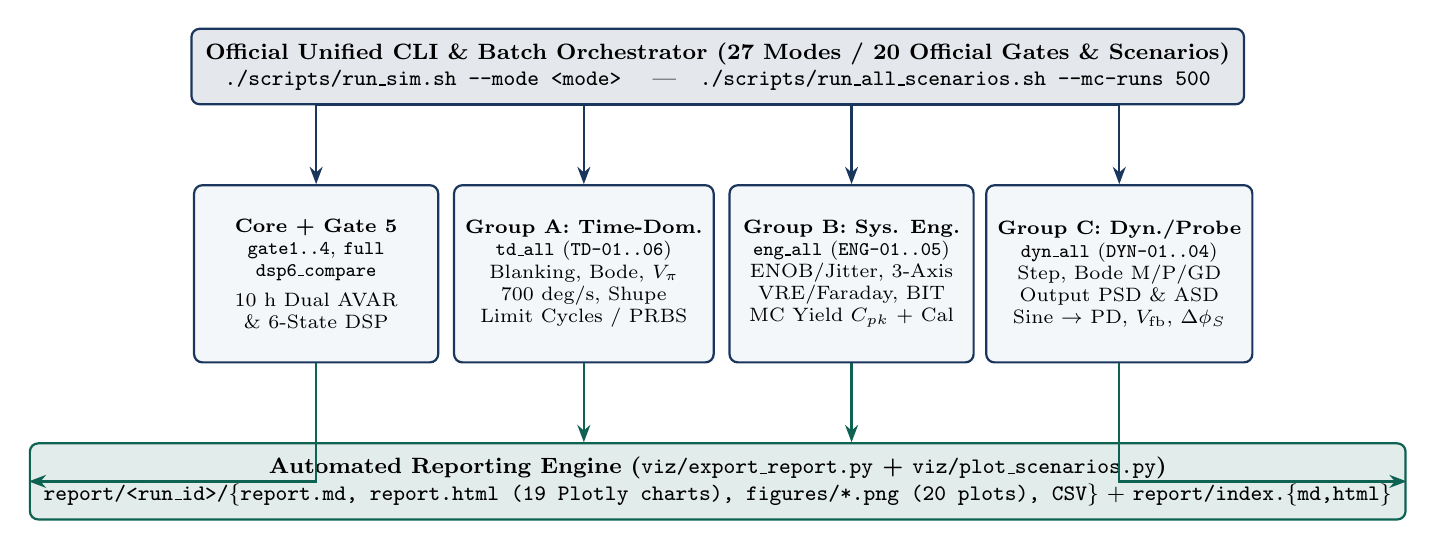
\begin{tikzpicture}[
    node distance=0.85cm and 0.6cm,
    cli/.style={rectangle,rounded corners=3pt,draw=NavyBlue,fill=NavyBlue!12,thick,align=center,font=\footnotesize,minimum width=12.4cm,minimum height=0.95cm,inner sep=5pt},
    grp/.style={rectangle,rounded corners=3pt,draw=NavyBlue,fill=SlateBg,thick,align=center,font=\scriptsize,minimum width=3.1cm,minimum height=2.25cm,inner sep=4pt},
    rep/.style={rectangle,rounded corners=3pt,draw=TealDark,fill=TealDark!12,thick,align=center,font=\footnotesize,minimum width=13.4cm,minimum height=0.95cm,inner sep=5pt},
    arr/.style={-{Stealth[length=2.2mm]},thick,NavyBlue},
    tarr/.style={-{Stealth[length=2.2mm]},thick,TealDark}
]
\node[cli] (top) {\textbf{Official Unified CLI \& Batch Orchestrator (27 Modes / 20 Official Gates \& Scenarios)}\\\texttt{./scripts/run\_sim.sh --mode <mode>} \quad|\quad \texttt{./scripts/run\_all\_scenarios.sh --mc-runs 500}};

\node[grp,below=1.0cm of top.south,xshift=-5.1cm] (core) {\textbf{Core + Gate 5}\\{\scriptsize\texttt{gate1..4}, \texttt{full}}\\{\scriptsize\texttt{dsp6\_compare}}\\[3pt]10 h Dual AVAR\\\& 6-State DSP};

\node[grp,below=1.0cm of top.south,xshift=-1.7cm] (td) {\textbf{Group A: Time-Dom.}\\{\scriptsize\texttt{td\_all} (\texttt{TD-01..06})}\\Blanking, Bode, $V_\pi$\\700 deg/s, Shupe\\Limit Cycles / PRBS};

\node[grp,below=1.0cm of top.south,xshift=1.7cm] (eng) {\textbf{Group B: Sys. Eng.}\\{\scriptsize\texttt{eng\_all} (\texttt{ENG-01..05})}\\ENOB/Jitter, 3-Axis\\VRE/Faraday, BIT\\MC Yield $C_{pk}$ + Cal};

\node[grp,below=1.0cm of top.south,xshift=5.1cm] (dyn) {\textbf{Group C: Dyn./Probe}\\{\scriptsize\texttt{dyn\_all} (\texttt{DYN-01..04})}\\Step, Bode M/P/GD\\Output PSD \& ASD\\Sine $\to$ PD, $V_{\text{fb}}$, $\Delta\phi_S$};

\node[rep,below=1.0cm of td.south,xshift=1.7cm] (out) {\textbf{Automated Reporting Engine (\texttt{viz/export\_report.py} + \texttt{viz/plot\_scenarios.py})}\\\texttt{report/<run\_id>/\{report.md, report.html (19 Plotly charts), figures/*.png (20 plots), CSV\}} + \texttt{report/index.\{md,html\}}};

\draw[arr] (top.south) -| (core.north);
\draw[arr] (top.south) -| (td.north);
\draw[arr] (top.south) -| (eng.north);
\draw[arr] (top.south) -| (dyn.north);
\draw[tarr] (core.south) |- (out.west);
\draw[tarr] (td.south) -- (out.north -| td.south);
\draw[tarr] (eng.south) -- (out.north -| eng.south);
\draw[tarr] (dyn.south) |- (out.east);
\end{tikzpicture}%
}
\caption{Official 5-Layer \texttt{IFOG-SIM-SPEC-005} Scenario Orchestration (20 Gates \& Scenarios), CLI Routing, and Automated Report Pipeline.}
\end{figure}

\subsection{Unified CLI Execution Reference Table}

\scriptsize
\begin{tabularx}{\textwidth}{@{}l l l X@{}}
\toprule
\textbf{ID} & \textbf{CLI Mode (\texttt{--mode})} & \textbf{Equations} & \textbf{Official Reproducible Command} \\
\midrule
ALL & \texttt{all\_scenarios} & \texttt{EQ-01..41} & \texttt{./scripts/run\_all\_scenarios.sh --run-id full\_all\_scenarios --mc-runs 500} \\
Gates 1--4 & \texttt{full} (\texttt{gate1..4}) & \texttt{EQ-01..30} & \texttt{./scripts/run\_sim.sh --mode full --run-id core\_4gates} \\
Gate 5 & \texttt{dsp6\_compare} & \texttt{EQ-31..34} & \texttt{./scripts/run\_sim.sh --mode dsp6\_compare --run-id gate5\_6state} \\
Group A & \texttt{td\_all} & \texttt{TD-01..06} & \texttt{./scripts/run\_sim.sh --mode td\_all --run-id td\_suite} \\
TD-01 & \texttt{td\_blanking} & \texttt{EQ-16,17,19} & \texttt{./scripts/run\_sim.sh --mode td\_blanking --run-id td01} \\
TD-02 & \texttt{td\_step\_sine} & \texttt{EQ-22,23,34} & \texttt{./scripts/run\_sim.sh --mode td\_step\_sine --run-id td02} \\
TD-03 & \texttt{td\_vpi\_shock} & \texttt{EQ-03,20,33,34} & \texttt{./scripts/run\_sim.sh --mode td\_vpi\_shock --run-id td03} \\
TD-04 & \texttt{td\_high\_rate} & \texttt{EQ-12,21,34} & \texttt{./scripts/run\_sim.sh --mode td\_high\_rate --run-id td04} \\
TD-05 & \texttt{td\_shupe\_shock} & \texttt{EQ-09,26} & \texttt{./scripts/run\_sim.sh --mode td\_shupe\_shock --run-id td05} \\
TD-06 & \texttt{td\_limit\_cycles} & \texttt{EQ-19,21} & \texttt{./scripts/run\_sim.sh --mode td\_limit\_cycles --run-id td06} \\
Group B & \texttt{eng\_all} & \texttt{EQ-35..41} & \texttt{./scripts/run\_sim.sh --mode eng\_all --run-id eng\_suite --mc-runs 500} \\
ENG-01 & \texttt{eng\_hw\_sizing} & \texttt{EQ-15,17,19,35} & \texttt{./scripts/run\_sim.sh --mode eng\_hw\_sizing --run-id eng01} \\
ENG-02 & \texttt{eng\_imu\_3axis} & \texttt{EQ-36} & \texttt{./scripts/run\_sim.sh --mode eng\_imu\_3axis --run-id eng02} \\
ENG-03 & \texttt{eng\_vre\_faraday} & \texttt{EQ-10,18,37,38} & \texttt{./scripts/run\_sim.sh --mode eng\_vre\_faraday --run-id eng03} \\
ENG-04 & \texttt{eng\_fault\_bit} & \texttt{EQ-39} & \texttt{./scripts/run\_sim.sh --mode eng\_fault\_bit --run-id eng04} \\
ENG-05 & \texttt{eng\_mc\_yield\_cal} & \texttt{EQ-40,41} & \texttt{./scripts/run\_sim.sh --mode eng\_mc\_yield\_cal --run-id eng05 --mc-runs 500} \\
Group C & \texttt{dyn\_all} & \texttt{EQ-06..23,31..34} & \texttt{./scripts/run\_sim.sh --mode dyn\_all --run-id dyn\_suite} \\
DYN-01 & \texttt{dyn\_step\_response} & \texttt{EQ-20,22,23,34} & \texttt{./scripts/run\_sim.sh --mode dyn\_step\_response --run-id dyn01} \\
DYN-02 & \texttt{dyn\_freq\_response} & \texttt{EQ-22,23,34} & \texttt{./scripts/run\_sim.sh --mode dyn\_freq\_response --run-id dyn02} \\
DYN-03 & \texttt{dyn\_output\_psd} & \texttt{EQ-15,19,26,33} & \texttt{./scripts/run\_sim.sh --mode dyn\_output\_psd --run-id dyn03} \\
DYN-04 & \texttt{dyn\_sine\_electro\_optic} & \texttt{EQ-06..19,21,31..34} & \texttt{./scripts/run\_sim.sh --mode dyn\_sine\_electro\_optic --run-id dyn04} \\
\bottomrule
\end{tabularx}
\normalsize

\section{Gate 5: Official 6-State Symmetric DSP (\texttt{EQ-31}--\texttt{EQ-34})}

Standard 4-state modulation uses instantaneous bias phases $[+\pi, +\alpha, -\pi, +\alpha]$ with non-zero DC mean $\alpha/2$ and peak swing $V_\pi$, causing RAM, PCB crosstalk, and quadratic MIOC distortion to rectify into rate bias. \texttt{IFOG-SIM-SPEC-005} standardizes the \textbf{anti-periodic 6-state symmetric modulation law} (\texttt{configs/baseline\_1km\_6state.json}, \texttt{dsp.mode = "6state"}):

\begin{equation}
\psi^{(6)} = \left[+\frac{\pi+\alpha}{2},\; -\frac{\pi+\alpha}{2},\; +\frac{\pi-3\alpha}{2},\; -\frac{\pi+\alpha}{2},\; +\frac{\pi+\alpha}{2},\; -\frac{\pi-3\alpha}{2}\right] \quad (\text{EQ-31})
\end{equation}
producing exact zero DC mean ($\sum_{s=1}^6 \psi_s = 0$), exact anti-periodicity ($\psi_{s+3} = -\psi_s$), and differential phases $\phi^{(6)} = [+(\pi-\alpha), -(\pi+\alpha), +(\pi-\alpha), -(\pi-\alpha), +(\pi+\alpha), -(\pi-\alpha)]$. At the optimal angle $\alpha^* = \pi/3$ (\texttt{EQ-32}), peak MIOC drive voltage falls by \textbf{33.3\%} ($\frac{2}{3}V_\pi$ vs $V_\pi$) while RAM, resistive/capacitive crosstalk, and quadratic MIOC $\gamma_{\text{nl}}V^2$ cancel identically in the rate demodulator. Three orthogonal demodulation channels (\texttt{EQ-33}) are extracted every $6\tau$ frame:
\begin{align}
e_\Omega^{(6)} &= (y_4 + y_5 + y_6) - (y_1 + y_2 + y_3) = 6 S_\alpha\,\Delta\phi_{\text{NR}}, \\
e_{V_\pi}^{(6)} &= 2(y_2 + y_5) - (y_1 + y_3 + y_4 + y_6) = 8\pi S_\alpha\,\epsilon_{V_\pi}, \\
e_{\text{asym}}^{(6)} &= (y_1 - y_3) + (y_6 - y_4) \quad \text{(online RAM/crosstalk/TIA-settling monitor)}.
\end{align}
Loop-1 applies anti-windup clamping $\Delta\phi_{\text{step}} \in [-\Delta\phi_{\max}, +\Delta\phi_{\max}]$ (\texttt{EQ-34}).

\small
\begin{tabularx}{\textwidth}{@{}l c c X@{}}
\toprule
\textbf{Gate 5 Benchmark Metric} & \textbf{4-State ($\alpha=\pi/4$)} & \textbf{6-State ($\alpha^*=\pi/3$)} & \textbf{Verified Gain} \\
\midrule
Peak MIOC Bias Voltage & $1.000\,V_\pi$ & $\mathbf{0.667\,V_\pi}$ & $-33.3\%$ drive voltage \\
Golden Static Phase Error & $7.72\times 10^{-17}\text{ rad}$ & $\mathbf{1.28\times 10^{-16}\text{ rad}}$ & Both $< 10^{-9}\text{ rad}$ (PASS) \\
Loop-2 Residual $\epsilon_{V_\pi,\text{eff}}$ & $2.44\times 10^{-15}$ & $\mathbf{1.31\times 10^{-11}}$ & Both $< 10^{-5}$ (PASS) \\
RAM + Crosstalk + $\gamma_{\text{nl}}$ Bias & $354.56\,^\circ/\text{h}$ & $\mathbf{5.04\times 10^{-5}\,^\circ/\text{h}}$ & $\mathbf{+136.94\text{ dB}}$ ($7.03\times 10^6\times$) \\
Online Monitor $e_{\text{asym}}$ RMS & N/A & $\mathbf{169.87\text{ counts}}$ & Detects impairment online \\
\bottomrule
\end{tabularx}
\normalsize

\section{Group A: 6 Time-Domain Simulation Scenarios (\texttt{TD-01}--\texttt{TD-06})}

All six scenarios execute directly on the unmodified Tier 2 physical core using the 64-byte sub-$\tau$ logger (\texttt{micro\_waveforms.bin}) and 64-byte cycle-accurate DSP register logger (\texttt{dsp\_trace.bin}):

\begin{enumerate}
    \item \textbf{\texttt{TD-01} --- Sub-$\tau$ Switching Transient \& ADC Blanking Alignment (\texttt{td\_blanking}):}
    Captures $P_{\text{det}}(t)$, $V_{\text{TIA}}(t)$, $V_{\text{drv}}(t)$, and \texttt{ADC\_strobe} at $K=32$ ($\Delta t_{\text{fast}} \approx 153\text{ ns}$) with LTF transients enabled. Sweeps $k_{\text{start}} \in [0, 12]$ against steady-state plateau error and verifies Butterworth settling $t_s(0.1\%)$ (\texttt{EQ-17}) and blanking ARW factor $1/\sqrt{\eta_b}$ (\texttt{EQ-19}).\\
    \emph{Verified Result:} TIA $t_s(0.1\%) = 174.1\text{ ns}$, optimal clean blanking start $k_{\text{start}}^* = 5$ (error drops from $2.98\%$ at $k=4$ to $<0.5\%$ at $k=5$), ARW penalty $\times 1.155$ (\textbf{PASS}).

    \item \textbf{\texttt{TD-02} --- Closed-Loop Step Response \& $-3\text{ dB}$ Bode Bandwidth (\texttt{td\_step\_sine}):}
    Applies a $0 \to 100^\circ/\text{s}$ step at $t=2.0\text{ ms}$ plus multi-frequency sinusoidal sweeps ($50\text{ Hz}$--$9\text{ kHz}$). Cross-checks measured $-3\text{ dB}$ bandwidth against the exact 1st-order frame-integrator closed-loop response $T_1(z_f) = K_{\text{tot}}/[z_f - (1-K_{\text{tot}})]$ (\texttt{EQ-34}).\\
    \emph{Verified Result:} Rise time $t_r = 0.22\text{ ms}$, overshoot $0.008\%$, steady error $2.66\times 10^{-7}\%$; measured $-3\text{ dB}$ BW $= \mathbf{2{,}540\text{ Hz}}$ vs analytical $\mathbf{2{,}354\text{ Hz}}$ ($7.8\%$ match, \textbf{PASS}).

    \item \textbf{\texttt{TD-03} --- Loop-2 $V_\pi$ Gain-Lock Transient Under $+5\%$ Thermal Shock (\texttt{td\_vpi\_shock}):}
    Injects a sudden $+5\%$ $\epsilon_{V_\pi}$ step at $t = 3.0\text{ ms}$ under steady $10^\circ/\text{s}$ rotation and tracks $G_{\text{DAC}}(t) \to 1/1.05$ and Loop-1 cross-coupling disturbance for both 4-state and 6-state DSP.\\
    \emph{Verified Result:} 4-state converges to $1.78\times 10^{-15}$ in $4.2\text{ ms}$ (Loop-1 peak $0.535^\circ/\text{s}$); 6-state converges to $1.68\times 10^{-11}$ in $6.3\text{ ms}$ with \textbf{2$\times$ lower Loop-1 disturbance ($0.269^\circ/\text{s}$)} (\textbf{PASS}).

    \item \textbf{\texttt{TD-04} --- High-Rate Dynamics ($300$--$700^\circ/\text{s}$), $2\pi$ Serrodyne Flyback \& Anti-Windup (\texttt{td\_high\_rate}):}
    Validates serrodyne ramp linearity and high-frequency modulo-$2\pi$ reset accuracy across $300$, $500$, and $700^\circ/\text{s}$, plus Loop-1 anti-windup clamping (\texttt{FLAG\_ANTI\_WINDUP}, \texttt{EQ-34}).\\
    \emph{Verified Result:} At $700^\circ/\text{s}$, RMS error $= \mathbf{0.00028\%}$ across $\mathbf{7{,}184}$ wraps ($179.6\text{ kHz}$, zero fringe slips); anti-windup clamps cleanly at $300.000^\circ/\text{s}$ with $200$ \texttt{FLAG\_ANTI\_WINDUP} events (\textbf{PASS}).

    \item \textbf{\texttt{TD-05} --- Real-Time Thermal Shupe Shock \& Extrapolative Filter (\texttt{td\_shupe\_shock}):}
    Drives Tier 2 with a real-time $\dot{T} = 2.0\text{ K/s}$ asymmetric thermal shock from Tier 1 (\texttt{shupe\_lut.bin}) and evaluates an extrapolative thermal-gradient compensation filter.\\
    \emph{Verified Result:} Peak Shupe bias $= \mathbf{1{,}483.61\,^\circ/\text{h}}$ ($r = 0.99998$ vs Tier 1 physics); thermal filter suppresses $\mathbf{99.74\%}$ ($3.85\,^\circ/\text{h}$ residual, \textbf{PASS}).

    \item \textbf{\texttt{TD-06} --- Quantization Limit Cycles (Idle Tones) \& PRBS Dither (\texttt{td\_limit\_cycles}):}
    Logs integer \texttt{adc\_code[n]}, \texttt{dac\_code[n]}, and \texttt{prbs\_bit[n]} at $\Omega_{\text{in}} = 0.005^\circ/\text{s}$ with 12-bit quantization to expose deadband limit cycles and verify reflected LFSR PRBS dither decorrelation.\\
    \emph{Verified Result:} Without dither, 12-bit quantization locks into only $\mathbf{3}$ unique DAC codes; enabling PRBS dither unlocks $\mathbf{1{,}595}$ unique codes and restores small-signal linearity (\textbf{PASS}).
\end{enumerate}

\section{Group B: 5 System Engineering \& Production Scenarios (\texttt{ENG-01}--\texttt{ENG-05})}

\begin{enumerate}
    \item \textbf{\texttt{ENG-01} --- Hardware Sizing \& Cost Trade-Off (\texttt{eng\_hw\_sizing}, \texttt{EQ-35}):}
    Runs three automated Tier 2 sweeps: (a) ADC/DAC ENOB sweep ($10, 12, 14, 16$-bit) to find the minimum passing resolution; (b) ADC sampling aperture jitter sweep ($0$--$10{,}000\text{ ps}$) governed by $\sigma_{V,\text{jit}} = |dV/dt|\sigma_{t,\text{jit}}$ and $\text{ARW}_{\text{tot}} = \sqrt{\text{ARW}_0^2 + \text{ARW}_{\text{jit}}^2}$; and (c) $3\times 3$ TIA $(R_f, C_{f,\text{opt}})$ vs SLD power $P_0$ Pareto trade-off.\\
    \emph{Verified Result:} Minimum passing ENOB $= \mathbf{12\text{-bit}}$; jitter increases ARW by $+2{,}216.3\%$ at $10\text{ ns}$; Pareto-optimal ARW $= \mathbf{1.412\times 10^{-4}\,^\circ/\sqrt{\text{h}}}$ (\textbf{PASS}).

    \item \textbf{\texttt{ENG-02} --- Concurrent 3-Axis IMU Shared-SLD \& Rail Crosstalk (\texttt{eng\_imu\_3axis}, \texttt{EQ-36}):}
    Invokes \texttt{./build/ifog\_sim --imu3axis} (\texttt{tier2\_sysc\_ams/src/imu\_3axis.cpp}), instantiating three concurrent full IFOG axes (\texttt{Axis\_X}, \texttt{Axis\_Y}, \texttt{Axis\_Z}) in one SystemC-AMS simulation coupled via \texttt{SharedPowerBus\_TDF} (shared SLD back-reflection + common power-rail droop with $-40\text{ dB}$ PSRR). Axis X spins at $500^\circ/\text{s}$ while Axis Y and Axis Z remain stationary.\\
    \emph{Verified Result:} Peak rail droop $= \mathbf{92.4\text{ mV}}$; stationary Axis-Y crosstalk drops from $\mathbf{40.63\,^\circ/\text{h}}$ (4-state) to $\mathbf{0.106\,^\circ/\text{h}}$ (official 6-state --- $\mathbf{+51.6\text{ dB}}$ rejection, \textbf{PASS}).

    \item \textbf{\texttt{ENG-03} --- Vibration Rectification Error (VRE) \& Magnetic Faraday / Mu-Metal Sizing (\texttt{eng\_vre\_faraday}, \texttt{EQ-37}, \texttt{EQ-38}):}
    Injects $1{,}500\text{ Hz}$ vibration ($g_{\text{rms}} \in [0..8]\,g$) through quadratic TIA nonlinearity $G_2 V^2$ to extract VRE $\Delta\Omega_{\text{VRE}} = K_{\text{VRE}} g_{\text{rms}}^2$ via Hann-windowed DC averaging; sweeps external magnetic field $B_{\text{ext}} \in [-5, +5]\text{ G}$ to measure Faraday sensitivity $S_B$ and required Mu-metal shielding $A_{\text{dB}} = 20\log_{10}(|S_B| B_{\max}/\Omega_{\text{budget}})$.\\
    \emph{Verified Result:} Total nonlinear VRE $= -0.3486\,^\circ/\text{h}/g^2$, pure $G_2$ quadratic VRE $= -0.0189\,^\circ/\text{h}/g^2$ ($\mathbf{R^2 = 0.9998}$); Faraday $S_B = \mathbf{0.18305\,^\circ/\text{h/G}}$ ($<10^{-8}\%$ vs theory), requiring $\mathbf{25.25\text{ dB}}$ Mu-metal shielding for $<0.01\,^\circ/\text{h}$ @ $1\text{ G}$ (\textbf{PASS}).

    \item \textbf{\texttt{ENG-04} --- 5-Mode Fault Injection \& Real-Time FPGA BIT/FDIR (\texttt{eng\_fault\_bit}, \texttt{EQ-39}):}
    Exercises \texttt{DigitalDSP\_SC::evaluate\_frame\_bit()} against five abrupt hardware/radiation faults injected at $t = 4.000\text{ ms}$: \texttt{sld\_drop\_50pct} (code 1, TTA $0.62\ \mu\text{s}$), \texttt{fiber\_break} (code 2, TTA $0.62\ \mu\text{s}$), \texttt{mioc\_electrode\_open} (code 3, TTA $30.00\ \mu\text{s}$), \texttt{adc\_saturation} (code 4, TTA $0.62\ \mu\text{s}$), and \texttt{dsp\_seu\_bitflip} (code 5, TTA $30.00\ \mu\text{s}$, automatic FDIR soft-rollback \texttt{recovered = True}). All $5/5$ detected within $< 200\ \mu\text{s}$ (\textbf{PASS}).

    \item \textbf{\texttt{ENG-05} --- Parallel Monte Carlo Production Yield ($C_{pk}$) \& $-40..+85^\circ\text{C}$ Virtual Thermal Calibration (\texttt{eng\_mc\_yield\_cal}, \texttt{EQ-40}, \texttt{EQ-41}):}
    Executes $N = 500$ parallel real Tier 1 + Tier 2 production builds with component tolerances ($\pm 5\%$ $V_\pi$, $\pm 10\%$ TIA GBW, log-normal fiber $h$, $\pm 20\%$ crosstalk) computing yield, 95\% Wilson CI, and $C_{pk}$; then sweeps 21 thermal calibration points ($[-40, +85]^\circ\text{C} \times \{-0.5, 0, +0.5\}\text{ K/s}$), exporting \texttt{virtual\_calibration\_dataset.csv} and verifying 2D polynomial \& 4-state EKF compensation.\\
    \emph{Verified Result ($N=500$):} Yield $= \mathbf{97.2\%}$ ($486/500$, 95\% Wilson CI $[95.36\%, 98.32\%]$, $C_{pk} = 0.604$); thermal drift RMS drops from $326.33\,^\circ/\text{h}$ to $\mathbf{0.050\,^\circ/\text{h}}$ ($\mathbf{99.98\%}$ poly reduction) and $\mathbf{0.170\,^\circ/\text{h}}$ ($\mathbf{99.95\%}$ 4-state EKF reduction) (\textbf{PASS}).
\end{enumerate}

\section{Group C: 4 Dynamic Response, Output PSD \& Electro-Optic Probe Scenarios (\texttt{DYN-01}--\texttt{DYN-04})}

Implemented in \texttt{tier3\_analysis/scenarios\_dynamic\_probe.py}, Group C adds dedicated closed-loop control characterization and internal electro-optic signal-chain probing using genuine Tier 2 C++ SystemC-AMS runs:

\begin{enumerate}
    \item \textbf{\texttt{DYN-01} --- Dedicated Closed-Loop Step Response (\texttt{dyn\_step\_response}):}
    Evaluates small-signal ($0 \to 10^\circ/\text{s}$) and large-signal tactical ($0 \to 100^\circ/\text{s}$, $\Delta\phi_S = 2.36\text{ rad}$) steps for 4-State vs Official 6-State DSP plus a Loop-1 gain sweep ($K_{\text{tot},1} \in \{0.15, 0.25, 0.45\}$), recording $t_d, t_r, t_{s,2\%}, t_{s,0.1\%}$, overshoot, tracking error convergence, and Sagnac $\Delta\phi_S(t)$ vs feedback $\Delta\phi_{\text{step}}(t)$.\\
    \emph{Verified Result:} 6-State $t_r = 0.206\text{ ms}$ ($10^\circ/\text{s}$) and $0.294\text{ ms}$ ($100^\circ/\text{s}$, $0.00\%$ overshoot, $0.0000\%$ steady-state error); gain sweep monotonically reduces $t_r$: $0.382 \to 0.206 \to 0.118\text{ ms}$ (\textbf{PASS}).

    \item \textbf{\texttt{DYN-02} --- Full Closed-Loop Frequency Response: Bode Magnitude, Phase \& Group Delay (\texttt{dyn\_freq\_response}):}
    Sweeps 15 log-spaced tones ($20\text{ Hz}$--$10\text{ kHz}$) in parallel for 4-State and Official 6-State DSP, extracting $|H(f)|$ [dB], unwrapped $\angle H(f)$ [deg], and group delay $\tau_g(f)$ [$\mu\text{s}$], overlaid against the exact half-frame-centered Z-domain FRF $H(f) = \frac{K_{\text{tot},1}}{1 - (1-K_{\text{tot},1})e^{-j2\pi f T_f}} e^{-j\pi f T_f}$.\\
    \emph{Verified Result:} 4-State BW $= \mathbf{2{,}544\text{ Hz}}$ ($\tau_{g,0} = 65.2\ \mu\text{s}$); 6-State BW $= \mathbf{1{,}642\text{ Hz}}$ ($\tau_{g,0} = 103.3\ \mu\text{s}$ vs theory $102.8\ \mu\text{s}$); exact $1.55\times$ ratio (\textbf{PASS}).

    \item \textbf{\texttt{DYN-03} --- Broadband Output Angular-Rate PSD, ASD \& Cumulative RMS Noise (\texttt{dyn\_output\_psd}):}
    Measures one-sided Welch output rate PSD $[(\text{deg/h})^2/\text{Hz}]$, ASD $[\text{deg/h}/\sqrt{\text{Hz}}]$, and cumulative RMS noise across $3\text{ Hz}$--$25\text{ kHz}$ for linear white-noise floor vs analytical \texttt{EQ-15}/\texttt{EQ-19} ARW, full-impairment 4-State, and full-impairment Official 6-State.\\
    \emph{Verified Result:} White-floor ARW $= \mathbf{0.000352\,^\circ/\sqrt{\text{h}}}$ vs analytical $0.000363\,^\circ/\sqrt{\text{h}}$ ($0.970\times$), HF roll-off $-13.5\text{ dB}$, and 6-State low-frequency ($5$--$40\text{ Hz}$) $1/f$ suppression $= \mathbf{+29.2\text{ dB}}$ (\textbf{PASS}).

    \item \textbf{\texttt{DYN-04} --- Sinusoidal Angular-Rate Input \& Internal Electro-Optic Probe (\texttt{dyn\_sine\_electro\_optic}):}
    Drives $\Omega_{\text{in}}(t) = 50^\circ/\text{s}\cdot\sin(2\pi\cdot 250\text{ Hz}\cdot t)$ ($16\text{ ms}$ + $8.2\text{ ms}$ full sub-$\tau$ $K=16$ trace) in Official 6-State DSP, directly plotting $\Omega_{\text{in}}$ vs $\Omega_{\text{out}}$ (THD/SFDR), Sagnac phase $\Delta\phi_S(t)$ vs feedback $\Delta\phi_{\text{fb}}(t)$ \& residual $\Delta\phi_{\text{err}}(t)$, MIOC serrodyne voltage $V_{\text{fb,MIOC}}(t)$ \& total $V_{\text{MIOC}}(t)$, Photodiode $P_{\text{PD}}(t)/I_{\text{PD}}(t)$ \& demodulated $\Delta P_{\text{PD}}(t)$, TIA $V_{\text{TIA}}(t)$, and $60\ \mu\text{s}$ sub-$\tau$ ADC blanking zoom.\\
    \emph{Verified Result:} Gain $= 0.9889$, phase lag $-9.36^\circ$, THD $= \mathbf{-67.5\text{ dB}}$, SFDR $= \mathbf{43.6\text{ dB}}$, $\Delta\phi_{S,\max} = 1.1800\text{ rad}$, $391$ $2\pi$ serrodyne resets, $r(\Delta P_{\text{PD,demod}}, \Delta\phi_{\text{err}}) = \mathbf{0.9960}$ (\textbf{PASS}).
\end{enumerate}

\section{Summary of Verified Official Scenario Acceptance Results}

\scriptsize
\begin{tabularx}{\textwidth}{@{}l l X c@{}}
\toprule
\textbf{ID} & \textbf{CLI Mode} & \textbf{Verified Real SystemC-AMS Quantitative Result} & \textbf{Status} \\
\midrule
Gate 5 & \texttt{dsp6\_compare} & 6s static err $1.28\times 10^{-16}\text{ rad}$, $\epsilon_{V_\pi}=1.31\times 10^{-11}$, RAM/xtalk gain $\mathbf{+136.94\text{ dB}}$, $-33.3\%$ $V_{\text{peak}}$ & \textcolor{TealDark}{\textbf{PASS}} \\
TD-01 & \texttt{td\_blanking} & TIA $t_s=174.1\text{ ns}$, optimal clean $k_{\text{start}}^*=5$ ($<0.5\%$ err), ARW $\times 1.155$ & \textcolor{TealDark}{\textbf{PASS}} \\
TD-02 & \texttt{td\_step\_sine} & Step $t_r=0.22\text{ ms}$, OS $0.008\%$, $-3\text{ dB}$ BW $= 2{,}540\text{ Hz}$ (theory $2{,}354\text{ Hz}$) & \textcolor{TealDark}{\textbf{PASS}} \\
TD-03 & \texttt{td\_vpi\_shock} & $+5\%$ $V_\pi$ shock: 6s conv $6.3\text{ ms}$ ($\epsilon=1.68\times 10^{-11}$), 2$\times$ lower Loop-1 peak ($0.269^\circ/\text{s}$) & \textcolor{TealDark}{\textbf{PASS}} \\
TD-04 & \texttt{td\_high\_rate} & $700^\circ/\text{s}$ RMS err $0.00028\%$, $7{,}184$ wraps ($179.6\text{ kHz}$), $200$ anti-windup clamps & \textcolor{TealDark}{\textbf{PASS}} \\
TD-05 & \texttt{td\_shupe\_shock} & Peak Shupe $1{,}483.61\,^\circ/\text{h}$ ($r=0.99998$), thermal filter suppresses $99.74\%$ & \textcolor{TealDark}{\textbf{PASS}} \\
TD-06 & \texttt{td\_limit\_cycles} & 12-bit quantization deadband unlocked by PRBS dither ($3 \to 1{,}595$ unique DAC codes) & \textcolor{TealDark}{\textbf{PASS}} \\
ENG-01 & \texttt{eng\_hw\_sizing} & Min ENOB $= 12\text{-bit}$, jitter $+2{,}216\%$ @ $10\text{ ns}$, Pareto ARW $1.412\times 10^{-4}\,^\circ/\sqrt{\text{h}}$ & \textcolor{TealDark}{\textbf{PASS}} \\
ENG-02 & \texttt{eng\_imu\_3axis} & Concurrent 3-axis IMU: rail droop $92.4\text{ mV}$, Axis-Y xtalk $40.63 \to 0.106\,^\circ/\text{h}$ ($+51.6\text{ dB}$) & \textcolor{TealDark}{\textbf{PASS}} \\
ENG-03 & \texttt{eng\_vre\_faraday} & Pure $G_2$ VRE $R^2=0.9998$; Faraday $0.183\,^\circ/\text{h/G}$; Mu-metal req. $25.25\text{ dB}$ & \textcolor{TealDark}{\textbf{PASS}} \\
ENG-04 & \texttt{eng\_fault\_bit} & $5/5$ faults detected (max TTA $30.0\ \mu\text{s} < 200\ \mu\text{s}$), SEU FDIR soft-rollback recovered & \textcolor{TealDark}{\textbf{PASS}} \\
ENG-05 & \texttt{eng\_mc\_yield\_cal} & $N=500$ MC Yield $= 97.2\%$ ($C_{pk}=0.604$); $-40..+85^\circ\text{C}$ Poly $99.98\%$ / EKF $99.95\%$ & \textcolor{TealDark}{\textbf{PASS}} \\
DYN-01 & \texttt{dyn\_step\_response} & 10 \& $100^\circ/\text{s}$ 4s/6s step ($t_r=0.206/0.294\text{ ms}$, OS $0.00\%$); $K_{\text{tot},1}$ monotonic speedup & \textcolor{TealDark}{\textbf{PASS}} \\
DYN-02 & \texttt{dyn\_freq\_response} & 15-pt Bode Mag/Phase/GD: 4s $2{,}544\text{ Hz}$ ($65.2\ \mu\text{s}$), 6s $1{,}642\text{ Hz}$ ($103.3\ \mu\text{s}$), ratio $1.55\times$ & \textcolor{TealDark}{\textbf{PASS}} \\
DYN-03 & \texttt{dyn\_output\_psd} & Output PSD ARW $0.000352\,^\circ/\sqrt{\text{h}}$ ($0.97\times$ EQ-15), 6s LF suppression $+29.2\text{ dB}$, HF $-13.5\text{ dB}$ & \textcolor{TealDark}{\textbf{PASS}} \\
DYN-04 & \texttt{dyn\_sine\_electro\_optic} & $50^\circ/\text{s}$ @ $250\text{ Hz}$: THD $-67.5\text{ dB}$, SFDR $43.6\text{ dB}$, $\Delta\phi_S=1.18\text{ rad}$, $391$ wraps, $r(\text{PD},\Delta\phi_{\text{err}})=0.9960$ & \textcolor{TealDark}{\textbf{PASS}} \\
\bottomrule
\end{tabularx}
\normalsize

\end{document}
